\chapter{Μηχανισμοί γενίκευσης και ομαδοποίησης}

Οι μέθοδοι γενίκευσης αποτελούν την πιο ευρέως διαδεδομένη τεχνική ανωνυμοποίσης. Η συγκεκριμένη προσέγγιση συνίσταται στην ομαδοποίηση των εγγραφών ή την αλλοίωση των γνωρισμάτων στα οποία ανφέρονται τα δεδομένα, μέσω της τροποποίησης της αντίστοιχης κλίμακας μεγέθους. Παρόλο που αυτή η μέθοδος μπορεί να αποβεί αποτελεσματική για την πρόληψη του εντοπισμού ενός προσώπου, δεν εξασφαλίζει αποτελεσματική ανωνυμοποίηση σε όλες τις περιπτώσεις. Για αυτό το λόγο έχουν παρουσιαστεί ειδικές και τεχνολογικά εξελιγμένες ποσοτικές προσεγγίσεις για την πρόληψη του συνδιασμού συνόλων δεδομένων, προς εξαγωγή συμπερασμάτων για μεμονομένα φυσικά πρόσωπα. 

Το κεφάλαιο αυτό ξεκινά με την παρουσίαση  του μοντέλου της $k$-ανωνυμίας. Στη συνέχεια περιγράφονται οι τεχνικές της $l$-διαφορετικότητας και $t$-εγγύτητας που επεκτείνουν της δυνατότητες της $k$-ανωνυμίας. Τέλος γίνεται  παρουσίαση σύγχρονων αλγορίθμων ανωνυμοποίησης που υλοποιούν αυτές τις μεθόδους.

\section{Θεμελείωση}

Όπως είδαμε στις προηγούμενες παραγράφους, μια από τις αποδοτικότερες λύσεις για την προστασία της ιδιωτικότητας των δεδομένων, αλλά ταυτόχρονα διατήρηση της χρησιμότητάς τους, είναι η ανωνυμοποίηση. Παρακάτω δίνουμε μερικούς ορισμούς και προτάσεις που θα χρησιμοποιήσουμε κατά την διάρκεια της διαδικασίας αυτής.

\begin{definition}-Περι συνόλων δεδομένων-
\begin{itemize}
\item Ένα \textbf{σύνολο δεδομένων}(\textlatin{dataset})  είναι μια πεπερασμένη συλλογή στοιχείων.

\item Κάθε στοιχείο του, ή εγγραφή, είναι μια διατεταγμένη λίστα τιμών και αντιστοιχεί σε ένα πρόσωπο, στο οποίο αναφέρονται τα δεδομένα τιμών για κάθε \textbf{γνώρισμα}(\textlatin{attribute}).

Το σύνολο δεδομένων το μοντελοποιούμε σαν μια πλειάδα στοιχείων-γραμμών $D=(x_1,x_2,...,x_n)$.



\item Η ανωνυμοποιημένη προβολή του $D$ συμβολίζεται ως $R$.
\item Ορίζουμε ως $A=A_1,A_2,...,A_r$ μια συλλογή από $r$ \textbf{γνωρίσματα}.
\item Συμβολίζουμε ως $t$ κάθε πλειάδα στο $R$.
\item Κάθε $t[A_i]$ με $i \in [1,r]$ εκφράζει την τιμή του γνωρίσματος $A_i$ στο $R$ για την $t$.
\item Συμβολίζουμε  $t[A]=(t[A_1],t[A_2],...,t[A_r])$.
\end{itemize}
\end{definition}
Θεωρητικά, ως ανωνυμοποίηση ενός συνόλου δεδομένων $D$ θεωρείται ένα σύνολο γενικέυσεων των γνωρισμάτων του, αποτελούμενο από μια ακριβώς γενίκευση ανά γνώρισμα του $D$. Αυτές οι γενικεύσεις μετασχηματίζουν το $D$ σε ένα νέο σύνολο δεδομένων $D'$. Επιπλέον, η διαδικασία της γενίκευσης είναι αυτή που δίνει το όνομά της στην οικογένεια μεθόδων που αναλύουμε στη συνέχεια.








\section{\textlatin{k}-ανωνυμία}
\label{sec:k}

Η μέθοδος της $k$-ανωνυμίας\footnote{\textlatin{k-anonymity}} είναι μια μη διαδραστική\footnote{Με τον όρο μη διαδραστική τεχνική εννοούμε ότι, μετά την εφαρμογή της, δημοσιοποιείται μια εξυγιασμένη προβολή της βάσης} τεχνική ιδιωτικότητας 
. Αρχικά, η $k$-ανωνυμία θεωρήθηκε ως πιθανή λύση στο πρόβλημα της ιδιωτικότητας, κυρίως λόγω της εννοιολογικής απλότητας και των αποτελεσματικών αλγορίθμων που εγγυώνται την εφαρμογή της. Δυστυχώς προέκυψε άμεσα ότι έχει ελλείψεις και δεν είναι σε θέση να προστατεύσει την ιδιωτικότητα όλων των ατόμων. Θα αναλύσουμε την μέθοδο της $k$-ανωνυμίας και στη συνέχεια, αφού δούμε τα κενά ασφαλείας, θα παρουσιάσουμε βελτιώσεις.

Η ιδέα πίσω από την $k$-ανωνυμία είναι ότι όταν δίνονται πληροφορίες για ένα άτομο από μια εξωτερική πηγή, όπως το όνομά του, η ημερομηνία γέννησής, ο ταχυδρομικός κώδικας, το φύλο κλπ., θα πρέπει να είναι αδύνατο να βρεθεί, με ακρίβεια, στο ανωνυμοποιημένο σύνολο-πίνακα η γραμμή-πλειάδα που αντιστοιχεί στο άτομο αυτό \textlatin{\cite{k}}. Διαισθητικά, η διαδικασία πρέπει να έχει ως αποτέλεσμα οποιοσδήποτε χρήστης της βάσης να μην είναι σε θέση να αποκτήσει πληροφορίες σχετικά με ένα συγκεκριμένο άτομο, αφού δεν μπορεί να εντοπίσει τις πληροφορίες του στη βάση δεδομένων. Αυτό μπορεί να επιτευχθεί με την κατάργηση ορισμένων γνωρισμάτων σε συνδυασμό με την τροποποίηση ορισμένων τιμών πριν την απελευθέρωση της βάσης δεδομένων.

Το πρώτο βήμα κατά τη δημιουργία της ανώνυμης βάσης δεδομένων $R$, είναι η κατάργηση γνωρισμάτων που προσδιορίζουν σαφώς τα άτομα. Είναι αυτά που συνήθως χρησιμοποιούμε ως πρωτεύοντα κλειδιά \footnote{\textlatin{primary keys}}: Γνωρίζοντας την τιμή ενός γνωρίσματος κάποιου ατόμου μας διευκολύνει να βρούμε, με μεγάλη πιθανότητα, την πλειάδα που αντιστοιχεί σε αυτό το άτομο, παραδείγματος χάρη η διεύθυνση, ο αριθμός δελτίου ταυτότητας, το όνομα, το τηλέφωνο, κλπ. Ωστόσο, υπάρχουν γνωρίσματα τα οποία, όταν λαμβάνονται μαζί, είναι δυνατό να ταυτοποιηθεί ένα άτομο. Μια τέτοια συλλογή γνωρισμάτων ονομάζεται \textlatin{quasi-identifier}. Σε γενικές γραμμές, ένα \textlatin{quasi-identifier} περιέχει γνωρίσματα τα οποία είναι πιθανόν να υπάρχουν και σε άλλες βάσεις.

Ο ακριβής ορισμός ενός \textlatin{quasi-identifier}\footnote{Σε διάφορα ελληνικά άρθρα έχει χρησιμοποιηθεί ο όρος «ψευδοαναγνωριστικό σύνολο», που είναι εμφανώς μακρυά από την αγγλική έννοια} βασίζεται στον διαχωρισμό μεταξύ ευαίσθητων και μη ευαίσθητων γνωρισμάτων. Η τιμή ενός ευαίσθητου γνωρίσματος πρέπει να παραμείνει μυστική, πράγμα που σημαίνει ότι σε μια ανωνυμοποιημένη βάση δεδομένων θα πρέπει να είναι αδύνατο να συνδεθεί μια ευαίσθητη τιμή (συγκεκριμένα, μια πλειάδα που περιέχει μια ευαίσθητη τιμή) σε ένα συγκεκριμένο άτομο. Με αυτόν τον τρόπο είναι αδύνατο να μάθει κανείς την ευαίσθητη τιμή ενός ατόμου από την ανωνυμοποιημένη βάση δεδομένων και έτσι διατηρείται η ιδιωτικότητα. Όλα τα γνωρίσματα εκτός των ευαίσθητων θα ονομάζονται μη ευαίσθητα. Θεωρείται επίσης ότι τα επιλεγμένα ευαίσθητα χαρακτηριστικά δεν εμφανίζονται σε άλλες βάσεις δεδομένων. Επομένως, όταν είναι γνωστή η τιμή ενός ευαίσθητου γνωρίσματος, δεν είναι δυνατόν να βρεθεί το άτομο που αντιστοιχεί σε αυτήν την τιμή, πράγμα που σημαίνει επίσης ότι ένα ευαίσθητο γνώρισμα δεν περιλαμβάνεται ποτέ σε ένα \textlatin{quasi-identifier}. Καταλήγουμε στο συμπέρασμα ότι ένα \textlatin{quasi-identifier} αποτελείται μόνο από μη ευαίσθητα γνωρίσματα.

\begin{definition}(\textlatin{quasi-identifier})\\
Ένα σύνολο από μη ευαίσθητα γνωρίσματα $Q={Q_1,Q_2,...,Q_r}$ καλείται \textlatin{quasi-identifier} για μια βάση δεδομένων $D$ αν υπάρχει $t \in D$ ώστε η πρόταση
$$ t=t' \lor t[Q]\neq t[Q'] $$ για κάθε $t'\in D$ να είναι ψευδής.
\end{definition}

Με άλλα λόγια, υπάρχει τουλάχιστον μια εγγραφή στην αρχική βάση δεδομένων που μπορεί να προσδιοριστεί μοναδικά χρησιμοποιώντας μόνο τιμές γνωρισμάτων του συνόλου $Q$. Δηλώνουμε το σύνολο όλων των \textlatin{quasi-identifier} με το σύμβολο $QI$.

Είναι προφανές ότι αν ένα γνώρισμα μπορεί να ορισθεί ως πρωτεύον κλειδί, τότε αποτελεί ένα \textlatin{quasi-Identifier}, όπως επίσης συλλογές γνωρισμάτων όπως \{ημερομμηνία γέννησης, Τ.Κ., φύλο\}. 

Στην συνέχεια θα αναφερθούμε σε ομάδες ατόμων τα οποία θα έχουν ίδιες τιμές για ένα σύνολο από \textlatin{quasi-identifiers}.

\begin{definition}(Κλάση Ισοδυναμίας)\\
Μια κλάση ισοδυναμίας για έναν πίνακα $R$ σε σχέση με τα γνωρίσματα στο $A$ είναι ένα σύνολο πλειάδων $E=\{t_1,t_2,...,t_i\} \in R$ για τα οποία $t_1[A]=t_2[A]=...=t_i[A]$. 
\end{definition}
Δηλαδή, η προβολή κάθε πλειάδας επί των γνωρισμάτων στο Α είναι ακριβώς ίδια.



\begin{figure} [h!]
\begin{center}
  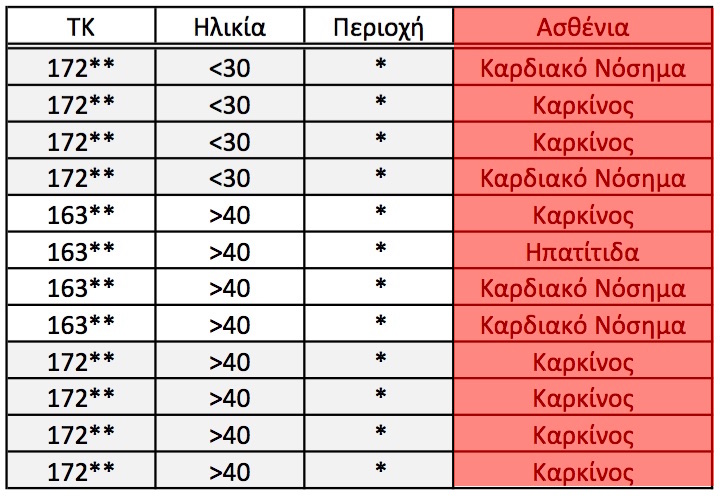
\includegraphics[scale=0.36]{images/k-anon.jpg}
  \caption{Ένα 4-ανώνυμο σύνολο δεδομένων}
  %\label{fig:boat1}
  \end{center}
\end{figure}

Στον παραπάνω πίνακα έχουμε 4 γνωρίσματα από τα οποία το ένα είναι ευαίσθητο (Ασθένια). Τα στοιχεία είναι ανωνυμοποιημένα. Επεμβαίνοντας στην Περιοχή και στα δυο τελευταία ψηφία του ΤΚ παρατηρούμε ότι δημιουργούνται τρεις ισοδύναμες κλάσεις, οι οποίες περιέχουν 4 εγγραφές οι κάθε μία.

Η $k$-ανωνυμία λειτουργεί εξασφαλίζοντας ότι υπάρχουν τουλάχιστον $k-1$ άλλα άτομα (δηλ. γραμμές στη βάση δεδομένων) που έχουν τις ίδιες τιμές για όλα τα \textlatin{quasi-identifiers}. Αυτό θα πρέπει να διασφαλίζει ότι αν ψάχνουμε για ένα συγκεκριμένο άτομο, θα έχουμε πάντα τουλάχιστον $k$ αποτελέσματα και έτσι δεν μπορούμε να προσδιορίσουμε την συγκεκριμένη πλειάδα.

\begin{definition}($k$-ανωνυμία)\\
Μια προβολή $R$ της βάσης $D$ θα είναι $k$-ανώνυμη αν για κάθε πλειάδα $t\in R$, και για κάθε \textlatin{quasi-identifier} $A\in IQ$, υπάρχουν τουλάχιστον $k-1$ άλλες πλειάδες $t_1,...,t_{k-1} \in R$ ώστε $t_1[A]=t_2[A]=...=t_{k-1}[A]$.
\end{definition}

Μια τεχνική για την επίτευξη $k$-ανωνυμίας είναι η γενίκευση γνωρισμάτων, η οποία αντικαθιστά τις τιμές των \textlatin{quasi-identifiers} με τιμές που είναι λιγότερο συγκεκριμένες αλλά σημασιολογικά ορθές. Ως αποτέλεσμα, περισσότερες εγγραφές θα έχουν το ίδιο σύνολο τιμών γνωριμάτων. Παρατηρούμε ότι ο παραπάνω πίνακας είναι 4-ανώνυμος, ενώ έχουμε \textlatin{quasi-identifier} το σύνολο γνωρισμάτων \{ΤΚ, Ηλικία, Περιοχή\}. Ο ορισμός της $k$-ανωνυμίας προϋποθέτει ότι ο υπεύθυνος της βάσης είναι σε θέση να αναγνωρίσει με ακρίβεια τα \textlatin{quasi-identifiers}. Ωστόσο, το έργο αυτό είναι πολύ δύσκολο στην εφαρμογή και είναι εύκολο να γίνει λάθος. Ειδικά ο διαχωρισμός ευαίσθητων και μη ευαίσθητων γνωρισμάτων μπορεί να είναι προβληματικός. Αυτό είναι σαφώς ένα από τα μειονεκτήματα της $k$-ανωνυμίας: Η υπόθεση ότι κάποιος είναι με ακρίβεια ικανός να βρει όλα τα \textlatin{quasi-identifiers} μοιάζει να είναι υπερβολικά απαιτητική.

\subsection{Επίτευξη \textlatin{k-anonymity}}

Υπάρχουν δυο κοινώς χρησιμοποιούμενες μεθόδοι για την επίτευξη της $k$-ανωνυμίας: 
\begin{itemize}

\item Η πρώτη είναι η τεχνική γενίκευσης - \textlatin{generalization}, όπου μια τιμή για ένα γνώρισμα μετατρέπεται σε μια γενικότερη και πιθανώς «αφηρημένη» τιμή. Παραδείγματος χάρη η τιμή του γνωρίσματος ΤΚ, όπου λείπουν τα δυο τελευταία ψηφία. Η απώλεια πληροφορίας είναι αναγκαστικά το τίμημα που πρέπει να πληρώσουμε ώστε να επιτευχθεί ιδιωτικότητα. 

\item Η δεύτερη μέθοδος είναι αυτή της απόκρυψης - \textlatin{suppression}. Όπως ορίζεται από την ίδια τη λέξη, εδώ η πληροφορία αποκρύπτεται εντελώς. Παραδείγματος χάρη η τιμή του γνωρίσματος Περιοχή. Η μέθοδος της απόκρυψης μπορεί να θεωρηθεί και σαν εφαρμογή της γενίκευσης, στον μέγιστο δυνατό βαθμό για κάποιο γνώρισμα. 
\end{itemize}
Μπορούμε τώρα να διατυπώσουμε το πρόβλημα της επίτευξης $k$-ανωνυμίας ελαχιστοποιώντας ταυτόχρονα τον αριθμό των γενικέυσεων ή αποκρύψεων που εφαρμόζονται. Αυτό θα είχε ως αποτέλεσμα τον βέλτιστο ανώνυμο πίνακα, όπου το βέλτιστο σημαίνει ότι η πληροφορία έχει παραμορφωθεί στο ελάχιστο, και έτσι μπορεί να θεωρηθεί ως η πιο χρήσιμη ανώνυμοποιημένη βάση δεδομένων. Ακόμα κι αν περιορίζουμε το πρόβλημα μόνο στην καταστολή των τιμών, μπορούμε να αποδείξουμε ότι το πρόβλημα βελτιστοποίησης είναι \textlatin{NP-Hard \cite{meyerson2004complexity}}. Επομένως στην πράξη εφαρμόζονται μόνο αλγόριθμοι προσέγγισης. Παρακάτω θα δείξουμε ότι η $k$-ανωνυμία αποτυγχάνει να προστατεύσει από πολλαπλές, πιθανώς ανεξάρτητες, προβολές.

\subsection{Επιθέσεις κατά της \textlatin{k}-ανωνυμίας}

Ενώ το μοντέλο της $k$-ανωνυμίας αποτελεί θεμελειώδη έννοια πάνω στην προστασία των δεδομένων, δεν εξασφαλίζει απόλυτα την ιδιωτικότητα σε συγκεκριμένες επιθέσεις. Όπως έχει αποδειχθεί, η $k$-ανωνυμία δεν εγγυάται πλήρως την μη αποκάλυψη της τιμής ευαίσθητων γνωρισμάτων των εγγραφών. Σε πολλές περιπτώσεις στατιστικών ερευνών απαιτείται η δημοσίευση των τιμών ενός ευαίσθητου γνωρίσματος ως έχουν, οι οποίες προφανώς δεν επηρεάζονται από την εφαρμογή $k$-ανωνυμοποίησης. Θεωρείται ότι εφόσον δεν μπορεί να ταυτοποιηθεί ένα άτομο με μια πλειάδα, δεν μπορεί να προκύψει συμπέρασμα για την τιμή που αυτό λαμβάνει για ένα ευαίσθητο γνώρισμα. Μπορεί, ωστόσο, κάποιος να συμπεράνει την τιμή του ευαίσθητου γνωρίσματος μιας ή περισσοτέρων ομάδων πλειάδων. Αν επιπλέον υπάρχει η δυνατότητα συνδυασμού κάποιων τιμών του \textlatin{quasi-identifier} που γνωρίζει ο επιτιθέμενος με κάποιες από αυτές που εμφανίζονται, θα μπορούσε να συμπεράνει την κλάση ισοδυναμίας που ανήκει η εγγραφή και πιθανότατα πληροφορίες σχετικά με το ευαίσθητο γνώρισμα. 

Οι ακόλουθες δύο κατηγορίες επιθέσεων αναλύθηκαν κατά την παρουσίαση της $l$-διαφορετικότητας \textlatin{ \cite{machanavajjhala2006ell}}.

\begin{itemize}
    \item \textbf{Eπίθεση ομοιογένειας}\\
    Αποδεικνύεται ότι εάν δεν υπάρχει διαφοροποίηση στην τιμή των ευαίσθητων γνωρισμάτων, παραβιάζεται η ιδιωτικότητα της εγγραφής. Εάν ο αριθμός των πλειάδων υπερβαίνει κατά πολύ τις πιθανές τιμές των ευαίσθητων χαρακτηριστικών, αυτό μπορεί να είναι μια κοινή κατάσταση. Παρατηρώντας τον προηγούμενο πίνακα βλέπουμε ότι αν ο επιτιθέμενος γνωρίζει ότι το άτομο που αναζητά βρίσκεται στη βάση δεδομένων, ενώ ταυτόχρονα ξέρει ότι είναι πανω απο 40 ετών και τα τρία πρώτα ψηφία του Τ.Κ. είναι 172, συμπεραίνει με βεβαιότητα ότι το άτομο πάσχει από καρκίνο. Ενώ η ταυτότητα του ατόμου προστατεύεται (ο επιτιθέμενος δεν γνωρίζει ποιά πλειάδα αντιστοιχεί στο άτομο), προκύπτει αποκάλυψη τιμής του ευαίσθητου γνωρίσματος.
    
    \item \textbf{Επίθεση με πρότερη γνώση}\\
    Ο επιτιθέμενος μπορεί επίσης να έχει γνώση σχετικά με τη κατανομή των ευαίσθητων τιμών. Στο προηγούμενο παράδειγμα, αν ο επιτιθέμενος γνωρίζει ότι το άτομο που αναζητά βρίσκεται στη βάση, ενώ ταυτόχρονα ξέρει ότι είναι κάτω απο 30 ετών, τότε η πλειάδα που αντιστοιχεί βρίσκεται στην πρώτη κλάση ισοδυναμίας. Αν επιπλέον γνωρίζει ότι είναι αθλητικός τύπος και προσέχει τη διατροφή του, εύκολα συμπεραίνει ότι είναι απίθανο να πάσχει απο καρδιακό νόσημα, άρα το άτομο έχει, με μεγάλη πιθανότητα, καρκίνο.
\end{itemize}

Μπορούμε να αποτρέψουμε την επίθεση ομοιογένειας διασφαλίζοντας ότι υπάρχει αρκετή ποικιλομορφία στις ευαίσθητες τιμές. Η προστασία από πρότερη γνώση είναι σχεδόν αδύνατη. Μπορούμε, ωστόσο, να δυσκολέψουμε τον επιτιθέμενο: Εάν υπάρχει μεγαλύτερη ποικιλία στις τιμές των ευαίσθητων γνωρισμάτων, θα χρειαστεί περισσότερη γνώση για την ανάκτηση της ακριβούς τιμής.
\clearpage










\section{\textlatin{l}-Διαφορετικότητα}

Το μοντέλο της $l$-διαφορετικότητας επεκτείνει την τεχνική της $k$-ανωνυμίας, έτσι ώστε να διασφαλιστεί ότι είναι αδύνατη η εφαρμογή επιθέσεων εξαγωγής συμπερασμάτων, εξασφαλίζοντας ότι κάθε γνώρισμα θα έχει τουλάχιστον $l$ διαφορετικές τιμές για κάθε κλάση ισοδυναμίας. 

\begin{definition}(Εντροπία $l$-διαφορετικότητας)\\
Για μια κλάση ισοδυναμίας $E$, έστω το $S$ το πεδίο τιμών των ευαίσθητων γνωρισμάτων και το $Pr [E, s]$ ο λόγος των εγγραφών στο $E$ που έχουν ευαίσθητη τιμή $s$, τότε το $E$ είναι $l$-διαφορετικό αν:
$$-\sum_{s\in S}Pr[E,s]log(Pr[E,s])\geq log(l)$$

\end{definition}

\begin{definition}
Ένα σύνολο δεδομένων είναι $l$-διαφορετικό αν όλες οι ισοδύναμες κλάσεις είναι $l$-διαφορετικές.
\end{definition}

Μιά απλούστερη εκδοχή του ορισμού είναι ότι κάθε κλάση ισοδυναμίας θα πρέπει να έχει τουλάχιστον $l$ διαφορετικές τιμές για το ευαίσθητο γνώρισμα (Διακριτή $l$-διαφορετικότητα).



\begin{figure} [h!]
\begin{center}
  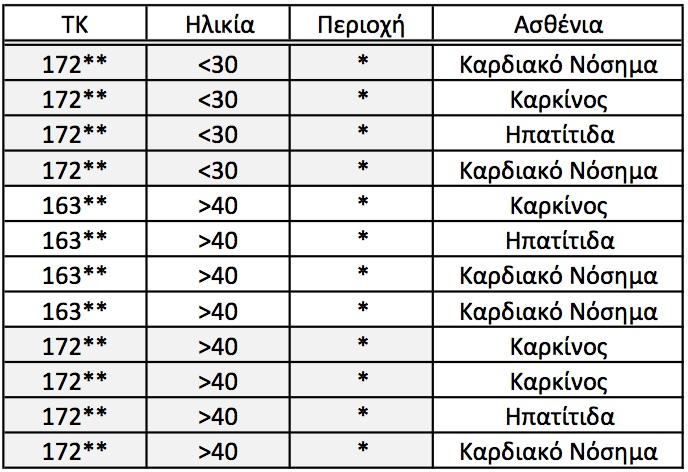
\includegraphics[scale=0.36]{images/k_anon.jpg}
  \caption{Ένα 3-διαφορετικό σύνολο δεδομένων}
  %\label{fig:boat1}
  \end{center}
\end{figure}

 Η σχέση στον ορισμό είναι σχεδόν η ίδια με την εντροπία του \textlatin{Shannon}, όπου οι πιθανότητες δίδονται τώρα ως κλάσματα συχνοτήτων των ευαίσθητων γνωρισμάτων. Όπως επισημάνθηκε στον παραπάνω ορισμό, για να υπάρχει $l$-διαφορετικότητα για κάθε κλάση ισοδυναμίας, η εντροπία ολόκληρου του πίνακα πρέπει να είναι τουλάχιστον $log (l)$. Κάποιες φορές αυτό μπορεί να είναι υπερβολικά περιοριστικό, καθώς η εντροπία ολόκληρου του πίνακα θα είναι αρκετά μικρή εάν κάποιες τιμές είναι πολύ συχνές. Αυτό οδηγεί στην ακόλουθη λιγότερο συντηρητική έννοια της $l$-διαφορετικότητας.
 
 \begin{definition}(Αναδρομική $(c,l)$-διαφορετικότητα)\\
 Έστω $m$ ο αριθμός των πιθανών τιμών ευαίσθητου γνωρίσματος σε μια κλάση ισοδυναμίας και $r_i$, με $i \in [1,m]$, το πόσες φορές η $i$-οστή συχνότερη τιμή εμφανίζεται στην κλάση $E$. Τότε η $E$ θα έχει $(c,l)$-διαφορετικότητα αν:
 $$r_1\leq c(r_l+r_{l+1}+...+r_m)$$
 \end{definition}
 
 
 \begin{definition}
Ένα σύνολο δεδομένων είναι $(c,l)$-διαφορετικό αν όλες οι ισοδύναμες κλάσεις είναι $l$-διαφορετικές.
\end{definition}
Η αναδρομική $(c, l)$-διαφορετικότητα εξασφαλίζει ότι η πιο συχνή τιμή δεν εμφανίζεται πολύ συχνά και οι λιγότερο συχνές τιμές δεν εμφανίζονται πολύ σπάνια.
 
 Γενικά, συμπεραίνουμε ότι η μέθοδος της $l$-διαφορετικότητας αντιμετοπίζει τις επιθέσεις ομοιογένειας, ενώ ταυτόχρονα δυσκολεύει τους επιτιθέμενους με πρότερη γνώση. Όσο υψηλότερη είναι η τιμή του $l$, τόσο περισσότερη γνώση απαιτείται για να αποκαλυφθεί η τιμή ενός ευαίσθητου χαρακτηριστικού ενός ατόμου. 
 
 
 
 \subsection{Επίτευξη \textlatin{l}-διαφορετικότητας}
 
 Η εισαγωγή της τεχνικής αυτής αποτελεί μια σημαντική βελτίωση της $k$-ανωνυμίας. Ωστόσο, παρατηρείται ιδιέταιρη δυσκολία στην εφαρμογή της.
 
 
 
 Ας θεωρήσουμε μια βάση δεδομένων μεγέθους $n=100000$ με ένα ευαίσθητο γνώρισμα δύο και μόνο πιθανών τιμών, το να έχει ή όχι τον ιό $HIV$. Έστω ότι το 99\% του δείγματος έχει την τιμή ΟΧΙ (είναι αρνητικοί στον ιό). Αν επιθυμούμε οποιαδήποτε τιμή προσέγγισης $l$-διαφορετικότητας, κάθε κλάση ισοδυναμίας θα πρέπει να έχει και τις δυο τιμές. Αυτό μεταφράζεται στην δημιουργία 1000 κλάσεων, που θα έχει ως αποτέλεσμα μεγάλη απώλεια πληροφορίας κατά την εφαρμογή γενίκευσης. Σημειώνουμε επίσης ότι επειδή η εντροπία του ευαίσθητου γνωρίσματος στον πίνακα είναι πολύ μικρή, η $l$-διαφορετικότητα μπορεί να επιτευχθεί μόνο εάν διαλέξουμε ένα αρκετά μικρό $l$, καθώς για μεγάλη τιμή θα ήταν στην πραγματικότητα αδύνατο να εξασφαλίσει διαφορετικότητα. Παρόλο που αυτό δεν αποτελεί ελάττωμα, το αναφέρουμε για να δείξουμε τη δυνητική δυσκολία να επιτύχουμε την $l$-διαφορετικότητα.
 
 \subsection{Επιθέσεις κατά της \textlatin{l}-διαφορετικότητας}
 
 Παρακάτω αναφέρουμε δυο είδη επιθέσεων κατά της μεθόδου αυτής.
 \begin{itemize}
     \item \textbf{Ασύμμετρη Επίθεση}\\
     Όταν η συνολική κατανομή είναι ασύμμετρη, η εφαρμογή $l$-διαφορετικότητας δεν εξασφαλίζει την μη αποκάλυψη τιμής ενός γνωρίσματος. Στο προηγούμενο παράδειγμα όπου το 99\% ενός πληθισμού έχει την τιμή ευαίσθητου γνωρίσματος ΟΧΙ, η αρχή της $l$-διαφορετικότητας επιτρέπει να υπάρχει μια κλάση ισοδυναμίας με ίσο αριθμό θετικών/αρνητικών στον ιό ατόμων. Παρατηρούμε ότι η ιδιωτικότητα κάθε ατόμου που ανήκει σε αυτή την κλάση χάνεται επειδή θεωρείται ότι έχει 50\% πιθανότητα να είναι θετικός στον ιό, αντί της πραγματικής 1\%.
     
     Ας θεωρήσουμε τώρα μια κλάση ισοδυναμίας που έχει 98 θετικές εγγραφές και μόνο 2 αρνητικές. Αυτή η κλάση είναι 2-διαφορετική και έχει μεγαλύτερη εντροπία από το σύνολο του πίνακα,   ικανοποιώντας έτσι κάθε $l$-διαφορετικότητα εντροπίας που κάποιος μπορεί να εφαρμόσει. Ωστόσο, ένα τυχαίο άτομο στην κλάση θα θεωρείται 98\% θετικός, αντί για 1\%. Στην πραγματικότητα, αυτή η κλάση ισοδυναμίας έχει ακριβώς την ίδια διαφορετικότητα με μια τάξη που έχει 2 θετικές και 98 αρνητικές εγγραφές, παρόλο που οι δύο κλάσεις παρουσιάζουν πολύ διαφορετικά επίπεδα κινδύνων ιδιωτικότητας.
     
     
     \item \textbf{Επίθεση ομοιότητας}\\
     Ένα άλλο πιθανό πρόβλημα παρουσιάζεται όταν οι τιμές ευαίσθητων χαρακτηριστικών είναι διακριτές αλλά σημασιολογικά παρόμοιες. Για παράδειγμα, μία κλάση ισοδυναμίας μπορεί να περιέχει διάφορους τύπους καρκίνων. Σε αυτή την περίπτωση γνωρίζουμε ότι όλοι στην ομάδα έχουν καρκίνο. Ένα άλλο παράδειγμα είναι ένα γνώρισμα που περιγράφει τον μισθό ενός συνόλου εργαζομένων. Κάθε άτομο σε μια κλάση μπορεί να έχει μια μοναδική τιμή, αλλά το συνολικό διάστημα μπορεί ακόμα να είναι μικρό. Ως εκ τούτου θα μπορούσαμε να μαντέψουμε με ακρίβεια το μισθό κάθε ατόμου λαμβάνοντας τον μέσο όρο στην κλάση.


 \end{itemize}









\clearpage
\section{\textlatin{t}-Εγγύτητα}

Μια βελτίωση της $l$-διαφορετικότητας που προσπαθεί να λύσει τα προβλήματα που παρουσιάσαμε ονομάζεται $t$-εγγύτητα. Εδώ προσπαθούμε να διασφαλίσουμε ότι η κατανομή ενός ευαίσθητου γνωρίσματος στην κλάση είναι ίδια με την κατανομή του σε ολόκληρο τον πληθυσμό. Αυτό έχει ως αποτέλεσμα τον ακόλουθο ορισμό.

\begin{definition}
Μια κλάση ισοδυναμίας $E$ θα έχει $t$-εγγύτητα εάν η απόσταση μεταξύ της κατανομής ενός ευαίσθητου γνωρίσματος στην κλάση αυτή και της κατανομής του γνωρίσματος σε ολόκληρο τον πίνακα δεν υπερβαίνει ένα κατώφλι $t$.
\end{definition}

\begin{definition}
Ένα σύνολο δεδομένων θα έχει $t$-εγγύτητα, αν όλες οι κλάσεις ισοδυναμίας του έχουν $t$-εγγύτητα.
\end{definition}

Το ακριβές μέτρο απόστασης που χρησιμοποιείται δεν έχει μεγάλη σημασία στο πλαίσιο της εργασίας αυτής. Παρόλο που η εγγύτητα είναι μια σαφής βελτίωση των προηγούμενων τεχνικών προστασίας της ιδιωτικότητας, θα δούμε στη συνέχεια ότι εξακολουθεί να είναι ευάλωτη σε μια επίθεση συνδεσιμότητας. Αυτό συμβαίνει κυρίως διότι η $t$-εγγύτητα - όπως επίσης kai οι προηγούμενες μέθοδοι - επικεντρώνονται σε στατικά δεδομένα που μένουν αμετάβλητα. Επομένως, περιορίζονται σε μια και μόνο δημοσίευση και δεν υποστηρίζουν την αναδημοσίευση μιας νέας προβολής της βάσης δεδομένων. 

Αυτό προκαλεί προβλήματα επειδή μπορεί να υπάρχει μια βάση δεδομένων, από διαφορετική εταιρία/οργανισμό, όπου είναι αποθηκευμένες σχεδόν οι ίδιες πληροφορίες.
Αν αυτός ο οργανισμός κοινοποιήσει μια ανώνυμοποιημένη βάση δεδομένων, η παραδοχή μιας «μοναδικής» δημοσίευσης παύει πλέον να ισχύει. Στην πραγματικότητα δηλαδή είναι αδύνατον να αποτρέψουμε πολλαπλές δημοσιεύσεις της ίδιας βάσης δεδομένων, και επομένως μηχανισμός ιδιωτικότητας που προυποθέτει μοναδική δημοσίευση, θεωρείται πρακτικά επισφαλής. 








\section{Επίθεση Τομής}

Μια επίθεση που δεν μπορεί να αντιμετοπίσει καμία από τις προαναφερθείσες τεχνικές, και ουσιαστικά καμία εκ των μεθόδων γενίκευσης, είναι η επίθεση τομής. 
Είναι μια ιδιαίτερη περίπτωση επίθεσης σύνθεσης, όπου συνδυάζονται δύο ή περισσότερες κοινοποιήσεις της βάσης δεδομένων ή επικαλυπτόμενες βάσεις, δημοσιευμένες από διαφορετικές οντότητες \textlatin{\cite{ganta2008composition}}. 
Η επίθεση τομής εξαρτάται από μια σημαντική ιδιότητα που μπορεί να διαθέτει ένας μηχανισμός προστασίας ιδιωτικότητας, εν ονόματει εντοπισμός (\textlatin{locatability}).

\begin{definition}(Εντοπισμός)\\
Έστω $Q$ το σύνολο των \textlatin{quasi-identifiers} τιμών μιας εγγραφής στην αρχική βάση δεδομένων $D$. Ένας μηχανισμός ανωνυμοποίησης $M$, που παράγει μια ανωνυμοποιημένη προβολή $R$ δεδομένης της βάσης $D$, ικανοποιεί την ιδιότητα του εντοπισμού αν κάποιος μπορεί να ταυτοποιήσει ένα σύνολο πλειάδων $\{t_1,t_2,...,t_k\}$ του $R$ που να αντιστοιχούν στο $Q$.
\end{definition}

Εν ολίγοις, δηλώνεται ότι, δεδομένων των τιμών των \textlatin{quasi-identifiers} ενός ατόμου, μπορούμε να βρούμε την κλάση ισοδυναμίας που ανήκει.

Όπως αναφέραμε και στην παράγραφο \ref{sec:k}, οι περισσότεροι αλγόριθμοι ανωνυμοποίησης παράγουν μια ανώνυμη βάση, δεδομένης την αρχικής. 
Η πλειοψηφία αυτών των μηχανισμών ικανοποιεί την ιδιότητα εντοπισμού, πράγμα που δεν ισχύει αναγκαστικά για όλους. 
Για αυτούς που δεν ικανοποιούν αυστηρά την ιδιότητα, τα πειράματα αποκαλύπτουν ότι απλές επιθέσεις συνδυαστικού τύπου μπορούν ακόμα να εντοπίσουν την κλάση ισοδυναμίας ενός ατόμου με ικανοποιητικού βαθμού πιθανότητα.
Η επίθεση τομής προϋποθέτει ότι ο μηχανισμός που χρησιμοποιείται για τη δημιουργία της ανώνυμης βάσης ικανοποιεί την ιδιότητα εντοπισμού.

Παρακάτω παρουσιάζουμε την αλγόριθμο της επίθεσης τομής:\\

\begin{algorithm}[H]
\textlatin{
 \KwData{$R_1,R_2,...,R_n$ \textgreek{Οι $n$ ανώνυμες προβολές}}
 $P$ \textgreek{ένα σύνολο ατόμων, κοινό στις $n$ δημοσιεύσεις}\\
 \For{i in P}{
  \For{j=1 to n}{
   $e_{ij} \longleftarrow GetEqClass(R_j,i)$\\
   $s_{ij} \longleftarrow SensitiveValueSet(e_{ij})$\\
   }{
   $S_i \longleftarrow s_{i1}\cap s_{i2} \cap ... \cap s_{in}$\\
  }
 }
 \Return $S_1, S_2,...,S_{|P|}$
 \caption{ Intersection Attack}}
\end{algorithm}

Έστω $R_1,R_2,...,R_n$ oι $n$ ανώνυμες προβολές μιας βάσης $D$. Έστω $P$ ένα επικαλυπτόμενο υποσύνολο ατόμων, των οποίων γνωρίζουμε την τιμή των 
\textlatin{quasi-identifiers}, που εμφανίζεται σε όλες τις δημοσιεύσεις.
Η συνάρτηση \textlatin{GetEqClass} επιστρέφει την κλάση ισοδυναμίας που ανήκει το άτομο, βασιζόμενη στις τιμές των \textlatin{quasi-identifiers} του.
Εφόσον υποθέσαμε ότι ο μηχανισμός προστασίας ιδιωτικότητας που παράγει τις ανωνυμοποιημένες προβολές $Rj$ ικανοποιεί την ιδιότητα εντοπισμού, αυτή η συνάρτηση υπάρχει σε κάθε περίπτωση.
Η συνάρτηση \textlatin{SensitiveValueSet} επιστρέφει το σύνολο των (ξεχωριστών) ευαίσθητων τιμών για τα άτομα σε μια δεδομένη κλάση ισοδυναμίας.

Αυτό που κάνει ο βρόχος είναι, από κάθε ανώνυμη προβολή να εξάγει το πιθανό σύνολο τιμών για το ευαίσθητο χαρακτηριστικό. Στη συνέχεια παίρνουμε την τομή όλων αυτών των συνόλων. Αν καταλήξουμε σε μία μόνο τιμή, μόλις αποκαλύψαμε το ευαίσθητο χαρακτηριστικό.

Έστω για παράδειγμα, ότι θέλουμε να εξάγουμε συμπέρασμα για την ασθένεια ενός ατόμου $a$, για το οποίο γνωρίζουμε ότι βρίσκεται στην ανωνυμοποημένη βάση $R$ και στην επίσης ανωνυμοποιημένη $B$. Έχουμε φτάσει στο συμπέρασμα με βάση την επεξεργασία της $R$,  ότι ο $a$ έχει Καρκίνο ή Διαβήτη, ενώ από την $B$, ότι πάσχει απο Καρδιακό νόσημα είτε από Καρκίνο. Προκύπτει λοιπόν το συμπέρασμα:

$$S_a={\{\text{Καρκίνος, Διαβήτης}\}}\cap \{\text{Καρδιά, Καρκίνος}\}=\{\text{Καρκίνος}\}$$

Προφανώς η ιδιωτικότητα του ατόμου $a$ έχει παραβιαστεί. Αυτή είναι μια «τέλεια παραβίαση» επειδή μπορούμε να συμπεράνουμε την ακριβή ευαίσθητη τιμή του ατόμου. Με άλλα λόγια ο επιτιθέμενος μαθαίνει την τιμή του ευαίσθητου γνωρίσματος ενός ατόμου με βεβαιότητα 100\%. Μια άλλη μορφή παραβίασης είναι η «μερική παραβίαση», η οποία μπορεί να συμβεί όταν ο επιτιθέμενος είναι σε θέση να συμπυκνώσει τις πιθανές ευαίσθητες τιμές σε λίγες μόνο, οι οποίες θα μπορούσαν να αποκαλύψουν πολλές πληροφορίες. 

Αν πάρουμε πάλι ως παράδειγμα την αποκάλυψη της ασθένειας του ατόμου $a$ και προκύψει μετά την τομή των αποτελεσμάτων:

$$S_a={\{\text{Υπέρταση, Ανεύρυσμα, Φλεβοθρόμβωση}\}}$$

προκύπτει το συμπέρασμα ότι το άτομο αυτό πάσχει από μια καρδιακή νόσο. Η πιθανότητα εύρεσης της νόσου σε αυτή την περίπτωση είναι 33\%.


Η επίθεση τομής εφαρμόστηκε σε δεδομένα ανωνυμοποιημένα με την μέθοδο της $k$-ανωνυμίας, $l$-διαφορετικότητας και $t$-εγγύτητας. Το συμπέρασμα ήταν ότι και οι τρεις μηχανισμοί αποτυγχάνουν να προστατεύσουν την ιδιωτικότητα όλων των ατόμων. Η $l$-διαφορετικότητα και η $t$-εγγύτητα αποδίδουν καλύτερα από την $k$-ανωνυμία, ωστόσο παρατηρούνται ακόμη περιπτώσεις παραβίασης. 
Κάτι που προκύπτει επιπλέον, είναι ότι για την $l$-διαφορετικότητα και $t$-εγγύτητα πρέπει να δημιουργηθούν μεγάλες κλάσεις ισοδυναμίας, με αποτέλεσμα μεγάλη απώλεια πληροφορίας.

Το συμπέρασμα λοιπόν είναι ότι όλες οι μεθόδοι γενίκευσης παρέχουν ικανοποιητική ιδιωτικότητα, προστατεύοντάς τα δεδομένα είτε από αποκάλυψη ταυτότητας, είτε από αποκάλυψη τιμής ευαίσθητου γνωρίσματος. Σε ιδιέταιρες καταστάσεις όμως, καμία από τις μεθόδους αυτές δεν μπορεί να αντιμετωπίσει την επίθεση τομής.

%Οι περισσότεροι μηχανισμοί ανωνυμοποίσησης που αναφέραμε στα προηγούμενα κεφάλαια έχουν εφαρμοστεί αλγοριθμικά




\clearpage
\section{Αλγόριθμοι Γενίκευσης}

Οι περισσότεροι μηχανισμοί ανωνυμοποίησης που παρουσιάσαμε στα προηγούμενα κεφάλαια, έχουν προσεγγιστεί κατά καιρούς με αλγορίθμους σε διάφορες γλώσσες προγραμματισμού, και έχουν αξιολογηθεί σε έρευνες. Στην παράγραφο αυτή επιδιώκουμε να συγκεντρώσουμε τις βέλτιστες και ταχύτερες προσεγγίσεις.

Τα τελευταία χρόνια έχουν δημοσιευτεί δεκάδες άρθρα που περιγράφουν και αναλύουν αλγορίθμους ανωνυμοποίσης συνόλων δεδομένων. 
Στόχος των αλγορίθμων αυτών είναι η δημιουργία μιας τροποποιημένης έκδοσης του συνόλου δεδομένων, έτσι ώστε η ιδιωτικότητα των εγγραφών να προστατεύεται επαρκώς, ενώ ταυτόχρονα, να διατηρείται η χρηστικότητα των δημοσιευμένων δεδομένων.



\subsection{\textlatin{Mondrian}}

Ο \textlatin{Mondrian} είναι ένας από τους κλασικότερους αλγορίθμους γενίκευσης και παρουσιάστηκε αρχικά ως εφαρμογή του μοντέλου της $k$-ανωνυμίας. Ως είσοδο δέχεται το σύνολο των αρχικών δεδομένων και επιστρέφει την βέλτιστη γενίκευση\footnote{Ως βλετιστη γενίκευση ορίζεται το ποσό γενίκευσης κατά το οποίο παρέχεται η μέγιστη δυνατή ιδιωτικότητα, εξασφαλίζοντας την ελάχιστη απώλεια πληροφορίας} του. 
Θεωρείται ένας από τους πιο σύγχρονους αλγορίθμους ανωνυμοποίησης και είναι ελκυστικός τόσο λόγω των λύσεων που παρέχει όσο και του χαμηλού χρόνου εκτέλεσης.

Η γενική ιδέα πίσω από τον αλγόριθμο είναι ένας \textlatin{top-down} διαχωρισμός των δεδομένων. Όλα τα αρχεία ανήκουν αρχικά στην ίδια κλάση ισοδυναμίας και αναδρομικά επιλέγεται μια διάσταση για να χωριστούν οι κλάσεις ισοδυναμίας, μέχρις ότου δεν υπάρχει καμία διάσταση στην οποία μπορεί να χωριστεί η κλάση για να παράγει έγκυρες $k$-ανώνυμες συστάδες. 

Ο αλγόριθμος ακολουθεί την εξής διαδικασία:
\begin{itemize}
    \item Ορίζονται οι περιοχές που καλύπτουν το χώρο των πεδίων τιμών  του \textlatin{quasi-identifier}
    \item Επιλέγεται η διάσταση με την οποία θα γίνει ο διαχωρισμός των κλάσεων. Υπάρχουν πολλοί τρόποι επιλογής, συνήθως όμως επιλέγεται η διάσταση με το μεγαλύτερο εύρος τιμών .
    \item Εφαρμόζεται ο διαχωρισμός κατά την παραπάνω επιλεγμένη διάσταση, βάσει της μέσης τιμής του αντίστοιχου γνωρίσματος, έτσι ώστε οι τιμές που είναι μικρότερες ή ίσες απο αυτήν να βρίσκονται στην αριστερή κλάση και οι υπόλοιπες να βρίσκονται στην δεξιά κλάση ισοδυναμίας.
    \item Η διαδικασία επαναλαμβάνεται για κάθε μία από τις δύο προκύπτουσες κλάσεις ισοδυναμίας αναδρομικά μέχρι να μην υπάρχει άλλη επιτρεπόμενη πολυδιάστατη τομή για διαχωρισμό σε καμία διάσταση. 
    \item Ως έξοδος, προκύπτει ο βέλτιστος διαχωρισμός και συνεπώς η κατάλληλη πολυδιάστατη γενίκευση που θα χρησιμοποιηθεί για να ανακωδικοποιηθούν τα δεδομένα.
\end{itemize}

Σε ψευδογλώσσα:


\begin{algorithm}[H]
\textbf{Συνάρτηση} $partition\_anon(P)$\\
\textlatin{
 \KwData{ \textgreek{Διαμ'εριση $P$}}
 \eIf{\textgreek{είναι αδύνατη περεταίρω πολυδιάστατη τομή της $P$}}{
   \Return $P$
   }{
   $dim \longleftarrow choosedimension(P)$\\
    $lhs \longleftarrow \{t\in \text{\textgreek{διαμεριση}}: t.dim = false\}$\\
     $rhs \longleftarrow \{t\in \text{\textgreek{διαμεριση}}: t.dim = true\}$\\
     \Return $partition\_anon(lhs)\cup partition\_anon(rhs)$
  }
 \caption{ Mondrian}}
\end{algorithm}



\subsection{Συσταδοποίηση (\textlatin{Clustering})}

Πέραν της χρήσης του $Mondrian$ για την ανωνυμοποίηση των δεδομένων, έχουν υιοθετηθεί μοντέλα από τον τομέα της εξόρυξης δεδομένων. Κλασικό παράδειγμα είναι η εφαρμογή αλγορίθμων συσταδοποίησης, η οποία θεωρείται πολλά υποσχόμενη μέθοδος.

Για την ανάπτυξη τέτοιων αλγορίθμων είναι απαραίτητο να ξεπεραστούν τα προβλήματα εγγύτητας με την αναζήτηση πλησιέστερων γειτόνων που χρησιμοποιεί κάθε φορά για να επιλέξει εγγραφές για συσταδοποίηση. Χρησιμοποιείται η εξής διαδικασία:
αντί να βρεθεί ο πλησιέστερος γείτονας μεταξύ όλων των εγγραφών, αρκεί να βρεθεί ο πλησιέστερος ανάμεσα σε κάποιο δείγμα ενός σταθερού αριθμού εγγραφών και να το δεχτεί. 



\subsection{ \textlatin{k - OPTIMIZE}}

Ο αλγόριθμος αυτός παρουσιάστηκε ως η βέλτιστη-ταχύτερη μέθοδος $k$-ανωνυμοποίησης.
Χρησιμοποιεί προτάσεις της Θεωρίας Γραφημάτων, ενω αποφεύγονται δαπανηροί αλγριθμικοί υπολογισμοί, όπως η ταξινόμηση \textlatin{\cite{Bayardo:2005:DPT:1053724.1054048}}.


Ο αλγόριθμος ξεκινά υπολογίζοντας μια τυχαία ανωνυμοποίηση του συνόλου. 
Στη συνέχεια εισέρχεται σε μια φάση γενίκευσης στην οποία οι τιμές αφαιρούνται διαδοχικά (πάντοτε επιλέγοντας εκείνη που βελτιώνει περισσότερο το χρονικό κόστος) έως ότου αυτό να μην μπορεί πλέον να βελτιωθεί.
Στη συνέχεια, μεταβαίνει σε μια φάση «εξειδίκευσης» στην οποία οι τιμές προστίθενται επαναληπτικά (και πάλι πάντα επιλέγοντας εκείνη που παρέχει τη μεγαλύτερη βελτίωση του κόστους) έως ότου δεν είναι δυνατή η βελτίωση. 
Ο αλγόριθμος εκτελεί επαναπληπτικά αυτές τις δύο φάσεις μέχρις ότου καμία φάση δεν είναι ικανή να βελτιώσει το \textlatin{score} (υποδηλώνοντας ότι επιτυγχάνεται τοπικό ελάχιστο).
Στο σημείο αυτό, καταγράφεται το κόστος ανωνυμοποίησης και ο αλγόριθμος επαναλαμβάνει ολόκληρη τη διαδικασία. Σημειώνεται ότι ο αλγόριθμος αυτός δεν έχει συνθήκες διακοπής και αντίθετα προσπαθεί συνεχώς να βελτιώσει την καλύτερη λύση που βρέθηκε μέχρι να σταματήσει ο χρήστης.






\begin{figure} [ht]
\begin{center}
  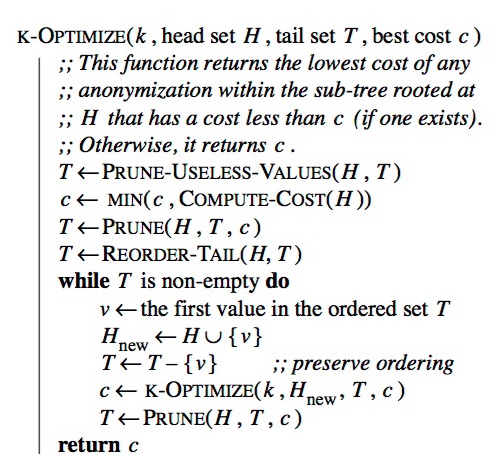
\includegraphics[scale=0.5]{images/optimize1.jpg}
  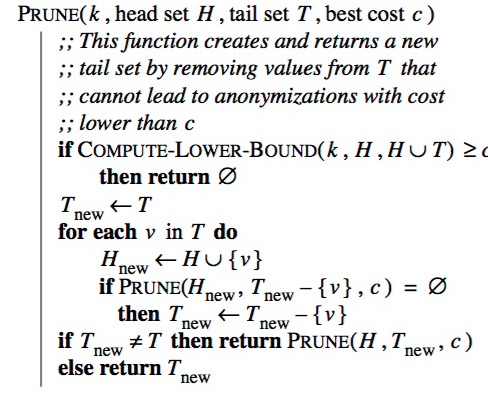
\includegraphics[scale=0.5]{images/optimize2.jpg}
  \caption{Μοντελοποίηση του αλγορίθμου \textlatin{k-optimize}  }
  %\label{fig:boat1}
  \end{center}
\end{figure}

Οφείλουμε να παρατηρήσουμε ότι αρκετοί από τους αλγορίθμους αυτούς χρησιμοποιούνται στην πράξη, ενώ διαθέσιμοι σε \textlatin{open-source} μορφή ύπάρχουν από πολλές πηγές, όπως \textlatin{Anonymization Toolbox}  από το Πανεπιστήμιο του Ντάλας και το \textlatin{ARX - Powerful Data Anonymization}, τα οποία υποστηρίζουν κυρίως τα μοντέλα $k$-ανωνυμίας και $l$-διαφορετικότητας. Στις βιβλιοθήκες ανωνυμοποίησης συνήθως συναντάμε και αλγορίθμους όπως ο \textlatin{Datafly} και ο \textlatin{Incognito}, οι οποίοι όμως δεν είναι τόσο αποτελεσματικοί όσο αυτοί που αναφέραμε παραπάνω.

Ένα βασικό σημείο στο οποίο υστερούν οι προαναφερθέντες αλγόριθμοι αποτελεί ο χρόνος εκτέλεσης, όπου κάποιες φορές είναι πιθανό να καθιστά αδύνατη την πρακτική εφαρμογή τους. Πρόσφατες μελέτες διερευνούν τη χρήση συμπληρωματικών μεθόδων ώστε να καταστούν οι μηχανισμοί αυτοί αποδοτικότεροι σε σχέση με την υπολογιστική τους πολυπλοκότητα, κάνοντάς τους φιλικότερους στη χρήση σε πρακτικές εφαρμογές. \textlatin{\cite{mohammadian2014fast}}